\documentclass{article}
\usepackage{tikz}
\usetikzlibrary{positioning, shapes.geometric}

\begin{document}

\section*{Generation (in red) and Verification (in blue) Methods for CRPs}

\subsection*{Verification is Successful if $q_{i} = q'_{i}$ and It Is Otherwise Failed}

\begin{figure}[h]
    \centering
    \begin{tikzpicture}[node distance=0.5cm and 1cm]
        % First box - Generation
        \node (gen) [draw, fill=red!20] {
            \begin{minipage}{0.45\textwidth}
                \centering
                $\ket{\psi_{in}}$ \\
                \begin{tikzpicture}[baseline=(current bounding box.center)]
                    \node[circle, draw, inner sep=1pt] (psi) {$\psi_{in}$};
                    \node[above right = 0.2cm and 0.3cm of psi] (label) {$\Lambda_U$};
                    \draw[-stealth] (psi) -- ++(0,-1) node[midway, left] {$m_i$};
                    \draw[-stealth] (psi) -- (label);
                    \draw[-stealth] (psi) -- ++(-2.5cm,0);
                \end{tikzpicture}
            \end{minipage}
        };
        % Second box - Verification
        \node (ver) [draw, fill=blue!20, right = of gen] {
            \begin{minipage}{0.5\textwidth}
                \centering
                $\ket{m'_i}$ \\
                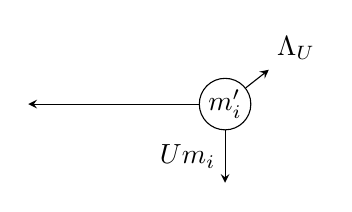
\begin{tikzpicture}[baseline=(current bounding box.center)]
                    \node[circle, draw, inner sep=1pt] (m) {$m_i'$};
                    \node[above right = 0.2cm and 0.3cm of m] (label2) {$\Lambda_U$};
                    \draw[-stealth] (m) -- ++(0,-1) node[midway, left] {$U\ket{m_i}$};
                    \draw[-stealth] (m) -- (label2);
                    \draw[-stealth] (m) -- ++(-2.5cm,0);
                \end{tikzpicture}
            \end{minipage}
        };
        % Connect the boxes
        \draw[-stealth] (gen.east) -- (ver.west);
    \end{tikzpicture}
    \captionsetup{justification=centering}
    \caption{Generation (red) and Verification (blue) methods for CRPs. Verification is successful if $q_{i} = q'_{i}$ and is otherwise failed.}
    \label{fig:crp_methods}
\end{figure}

\end{document}